\documentclass[11pt]{article}
\usepackage[margin=1in]{geometry}
\usepackage{amsmath,amssymb,amsthm,booktabs,microtype,graphicx}
\usepackage[hidelinks]{hyperref}
\newtheorem{theorem}{Theorem}
\newtheorem{corollary}[theorem]{Corollary}
\newcommand{\tr}{\operatorname{tr}}
\newcommand{\vol}{\operatorname{vol}}
\newcommand{\F}{\mathcal F}
\title{How many steps of label diffusion are fixed by local neighborhood counts?}
\author{Yunjie Guo \and Hanqing Yang\thanks{Corresponding author. Email: \texttt{hanqing.yang189@gmail.com}.}}
\date{Independent Researcher, Suzhou, China}
\newcommand{\primaryrows}{
Karate & 34/78 & 75.86 & 73.37--77.42 & 73.00--79.30 & 50.07 & 1.91 \\
Football & 115/613 & 39.05 & 38.66--39.34 & 37.96--41.17 & 8.88 & 0.14 \\
Cornell & 183/277 & 17.72 & 12.23--22.39 & 10.92--24.47 & 28.10 & 2.16 \\
Texas & 183/279 & 12.67 & 8.56--16.47 & 7.23--18.45 & 27.41 & 1.70 \\
Wisconsin & 251/450 & 23.63 & 16.08--28.98 & 14.71--30.68 & 29.92 & 1.52 \\}
\newcommand{\depthrows}{
Karate & 7.250 & 0.000 & 46 & 2 & 2 & -0.615 & +0.459 \\
Football & 0.765 & 0.000 & 249 & 0 & 0 & -0.022 & +0.030 \\
Cornell & 12.998 & 0.016 & 200 & 12 & 2 & -0.513 & +0.289 \\
Texas & 9.362 & 0.035 & 186 & 17 & 0 & -0.269 & +0.272 \\
Wisconsin & 15.747 & 0.019 & 371 & 20 & 8 & -0.259 & +0.178 \\}

\begin{document}
\maketitle

\begin{abstract}
A network randomization can preserve every vertex's local label counts and still alter the movement of a random walker between label classes. We determine the first time at which this ambiguity can occur. In an undirected graph with fixed depth-$r$ color-refinement signatures at each named vertex, the stationary joint distribution of the initial and final labels is identical through time $2r$. Time $2r+1$ is sharp even for two connected cycles related by one edge switch. At that first possible time of disagreement, every linear contrast of the joint distribution has attainable extrema given by independent weighted degree-constrained subgraph problems. Applied to three university web graphs at depth one, the range of three-step label agreement spans 7.91--12.91 percentage points, although every feasible value stays below its independent-label reference. At a common five-step horizon, a second neighborhood round reduces the widths on these graphs to at most 0.035 percentage points. The bounds separate uncertainty about a diffusion statistic from uncertainty about the edges themselves.
\end{abstract}

\section{Introduction}
Suppose a network data release reports, for every vertex, its category and the number of incident links to each category. One can recover exactly the probability that a randomly oriented edge has identically labeled ends. Can one also recover the probability that the two ends of a walk of length two, three, or five have the same label? A related question arises when evaluating structure-preserving randomized controls. A diffusion statistic may agree across every control because the imposed constraints force agreement. Conversely, a narrow sample range may coexist with substantially different attainable values.

We study the joint distribution of the start and end labels of a stationary random walk on an undirected simple graph. Its trace is the same-label probability. Subtracting the independent-label reference gives the fixed-time trace of the clustered autocovariance used in Markov stability \cite{stability}. The graph may be disconnected. We specify the degree-proportional stationary start throughout. Labels are observed metadata. The estimand concerns movement between these categories, including walks that backtrack.

Two existing lines of work provide the ingredients. The neighborhood structure configuration model (NeSt) of Stamm et al.\ \cite{nest} preserves successively refined colors and samples from the resulting graph families using switches within color blocks. Their analysis studies finite iterations of centrality computations. Color refinement also characterizes information in rooted tree unfoldings and tree homomorphism counts \cite{dell}. In a different optimization setting, Winterbach et al.\ \cite{winterbach} compute extreme degree assortativities by assigning edge scores and solving a weighted perfect $b$-matching. Higher-order mixing is also relevant to graph learning under heterophily \cite{zhu}, where distinct-distance neighborhoods are often used. Here repeated vertices in a walk contribute according to their transition probabilities.

Our contribution concerns what these local constraints identify about a \emph{two-ended, degree-normalized} observable. Reversibility doubles the guaranteed time horizon. A single switch on a cycle proves the guarantee optimal for each depth. At the following time the unknown transition appears only once, between two known diffused signals. This gives both an optimization formula for the full label mixing matrix in any linear direction and a local explanation of the changes that control it. The data analysis evaluates magnitudes, signs and ambiguity at a common time horizon. It uses the established NeSt family and standard matching machinery.

\section{Local information and the sharp horizon}
Let $G=(V,E)$ be an undirected simple graph with degrees $d_v>0$, $m=|E|$, adjacency $A$, $D=\operatorname{diag}(d)$, $P=D^{-1}A$ and $\Pi=D/(2m)$. The $v$th row of $F$ is the indicator vector of the observed label $c_0(v)$. Define a signature recursively by
\[
 c_{j+1}(v)=\big(c_j(v),\,\{\!\{c_j(u):u\sim v\}\!\}\big).
\]
The multiset records multiplicities. Colors have shared meanings across graphs, for example by retaining the tuples themselves. For $r\ge1$, the family $\F_r(G)$ consists of simple graphs on the same named vertices, with the same initial labels and the same $c_r(v)$ at each vertex. Recording just a histogram of colors gives a different observation model. Equivalently, fix the reference partition by $c_{r-1}$ and the counts $k_{vb}$ of neighbors of $v$ in each part $b$. Indeed, every coarser partition is a union of these parts. Induction from the known initial labels then reconstructs every signature through round $r$. In particular $D$, $m$ and $\Pi$ are common to the family.

Write $M_t=F^\top\Pi P^t F$. Entry $(i,j)$ is the probability of a walk beginning in class $i$ and ending in class $j$. Its trace $h_t$ lies in $[0,1]$. With $\pi_v=d_v/(2m)$ and $\mu=F^\top\pi$, the centered trace is $h_t-\|\mu\|^2$. The reference $\|\mu\|^2$ is the agreement of two independent draws from the fixed stationary label distribution.

\begin{theorem}[Finite horizon and sharpness]\label{thm:horizon}
Over $\F_r(G)$, the entire matrix $M_t$ is fixed for $0\le t\le 2r$. For every $r\ge1$ there exist two labeled connected cycles in the same family, differing by one degree-preserving switch, with distinct $h_{2r+1}$.
\end{theorem}
\begin{proof}
Set $Q_j=P^jF$. Its row at $v$ depends only on $c_j(v)$. At $j=0$ this is the definition. The induction step averages the previous rows using the neighbor multiplicities and their sum, $d_v$. Thus $Q_j$ is fixed through $r$. Detailed balance gives $\Pi P=P^\top\Pi$. With $a+b=t$ and $a,b\le r$,
\[
                    M_t=Q_a^\top\Pi Q_b .
\]
This proves the first assertion, including odd times below the cutoff.

For sharpness, take the cycle on $N=2L$ vertices numbered modulo $N$, where $L=8r+8$. Mark just $0$ and $L$ with a second label. Remove the edges $(r,r+1)$ and $(L+r,L+r+1)$ and join $r$ to $L+r$ and $r+1$ to $L+r+1$. Removing the original edges leaves two paths. Each new edge connects the paths, yielding one cycle. All four endpoints originally have the same depth-$(r-1)$ color: no marked vertex occurs within that radius, and degrees are two. Thus the switch preserves each vertex's counts into the reference color parts and hence its depth-$r$ signature.

Put $k=2r+1$. Before the switch the two marks are at distance $L>k$. After the switch their shorter connecting arc has length $k$. Each oriented shortest walk has probability $2^{-k}$. The diagonal return probabilities to each mark agree since both underlying graphs are $N$-cycles. If $p$ denotes the probability of starting and ending marked, $h_k=1-2(2/N)+2p$ by stationarity. The two additional oriented walks therefore increase $h_k$ by $4/(N2^k)>0$.
\end{proof}

\begin{figure}[ht]
\centering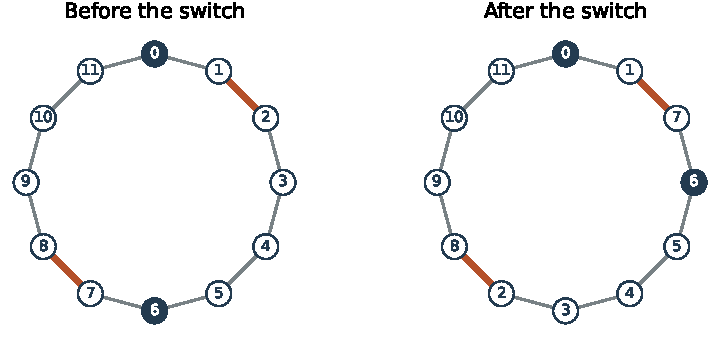
\includegraphics[width=.61\linewidth]{cycle.pdf}
\caption{A depth-one example on 12 vertices. The marks are vertices 0 and 6. The two highlighted edges on the left are replaced by those on the right. Every vertex keeps its count of marked neighbors. The distance between the marks falls from six to three, increasing three-step same-label agreement by $1/24$.}
\end{figure}

The two example graphs have identical uncolored spectra. Their labeled spectral measures differ. One cannot replace stationary averaging by a fixed starting vertex in the doubling argument: the split uses the stationary inner product. Individual rows of $P^tF$ have the shorter guaranteed horizon $r$.

\section{Attainable bounds at the following time}
Put $k=2r+1$ and let $q_v^\top$ denote row $v$ of the known $Q_r$. For a symmetric matrix $B$ define $H_B=\tr(B^\top M_k)$. The identity matrix returns $h_k$. Symmetric contrasts suffice because reversibility makes $M_k$ symmetric.

\begin{theorem}[Directional endpoints]\label{thm:ext}
For each unordered pair of $c_{r-1}$ parts $(a,b)$, form candidate edges between distinct vertices in the required parts. Omit vertices with zero incidence quota towards the opposite part. Let $\mathcal X_{ab}$ comprise their binary edge vectors meeting each vertex's quota towards that part. With $w_{uv}=q_u^\top Bq_v$,
\[
\min_{\F_r(G)} H_B=\frac{1}{m}\sum_{a\le b}
   \min_{x\in\mathcal X_{ab}}\sum_{uv} w_{uv}x_{uv},\qquad
\max_{\F_r(G)} H_B=\frac{1}{m}\sum_{a\le b}
   \max_{x\in\mathcal X_{ab}}\sum_{uv} w_{uv}x_{uv}.
\]
Both endpoints have simple-graph witnesses. These supports specify the convex hull of the attainable matrices.
\end{theorem}
\begin{proof}
Splitting the walk gives $M_k=Q_r^\top A Q_r/(2m)$. Each undirected edge contributes the two ordered terms, yielding $w_{uv}/m$ after contraction. Constraints in separate blocks concern disjoint edge variables and fix different entries of the vertex quota vector. Their feasible sets form a Cartesian product. A union of block optimizers is simple and satisfies every quota. Conversely every member of the family restricts to such a feasible tuple. The last conclusion follows from separation for a finite set's convex hull.
\end{proof}

Cross-part optimizations are capacitated bipartite matchings. Same-part optimizations are simple perfect $b$-matchings with prescribed degrees. Omitting the binary constraints from a same-part incidence formulation can introduce fractional odd cycles. Our reference implementation uses a binary optimization model, with at most $\binom{|V|}{2}$ candidate edges overall. A dense color block can dominate computation. An endpoint refers to one contrast at a time: entrywise bounds alone cannot in general be achieved by a single graph, and a finite family can have gaps between its extremal values.

\paragraph{A switch criterion for rigidity.}
In an admissible block switch $(u,v),(x,y)\mapsto(u,y),(x,v)$ on distinct vertices, the contrast changes by
\[
                 (q_u-q_x)^\top B(q_y-q_v)/m .
\]
Consequently the first unprotected contrast is fixed if and only if this product vanishes for every switch feasible \emph{somewhere} in the family. To see sufficiency, the realizations in each simple or bipartite degree block are connected by degree-preserving switches \cite{switch,nest}. Applying one block's path at a time connects the whole family. Necessity follows by evaluating the two realizations on opposite sides of any switch. The formula can also enumerate the exact range achievable from the observed graph with at most one switch. In particular a variable graph can have a fixed statistic.

\paragraph{A fast outer bound for the trace.}
Create one stub for every incident edge in each block and attach its endpoint's vector $q_v$. In a cross-part block and for each label coordinate separately, sort the left and right stub values. Pairing in like order maximizes the scalar product and opposite order minimizes it by the rearrangement inequality. Sum the coordinate products. In a same-part block use two copies of the combined stub list, then divide by two because each edge contributes twice. Every graph induces a permutation of these stubs. Allowing arbitrary permutations per coordinate can introduce loops, repeated edges or incompatible coordinate matchings. The resulting values enclose the exact edge sums and can be computed in $O(Cm\log(2m))$ time for $C$ labels, without constructing a dense candidate graph. If the outer endpoints coincide, the observed graph attains both.

\paragraph{Consequence for continuous time.}
Let $\mathcal H(s)=\tr(F^\top\Pi e^{s(P-I)}F)$ and let $W$ be the sharp width of $h_k$ above. Put $p_j=e^{-s}s^j/j!$ and $R=\sum_{j>k}p_j$. The width of $\mathcal H(s)$ across the family lies between $\max(0,p_kW-R)$ and $p_kW+R$. Indeed the earlier terms cancel in every difference and each later $h_j$ lies in $[0,1]$. For the lower bound evaluate the two graphs attaining the $h_k$ extrema. Thus $W/k!$ is the leading coefficient of the width at order $s^k$ as $s\downarrow0$. This gives the discrete frontier a short-time interpretation without optimizing a matrix exponential.

\section{Evaluation}
We used Zachary's club split \cite{zachary}, the conference labels of the 2000 US college football schedule \cite{football}, and the five webpage categories in the Cornell, Texas and Wisconsin WebKB graphs released with Geom-GCN \cite{pei}. The three campuses share a data collection and label scheme. Each graph is undirected and unweighted after merging reciprocal hyperlinks, discarding loops and omitting isolates. We fixed the NetworkX release for karate and recorded checksums of the football archive and all six WebKB input files. No classifier, feature matrix or fitted label was needed. The five case studies describe these particular graphs.

For each depth in $\{1,2,3\}$ we solved the minimum and maximum for the trace, constructed the witnessing edge sets and recomputed the probability by walking on each witness. We compared the bounds with the stub relaxation and the span of three constrained-switch chains initialized at the original graph. Each chain used 20 warm-up sweeps and 32 recorded sweeps, with $m$ proposals per sweep. Eligible blocks with at least two edges were selected uniformly, then two distinct edges uniformly within the block. Within one color part we chose between the two orientations with equal probability. Rejections leave the current state in place. The 96 values characterize this computation budget. No mixing-time or uniform independent sampling assumption enters the comparison.

\begin{table}[ht]
\centering\small
\caption{Three-step same-label agreement with one round fixed. Observed value, feasible endpoints and independent-label reference are percentages. Sample and stub columns are widths in percentage points.}
\begin{tabular}{lrrrrrrrr}
\toprule
Graph & $n/m$ & $C$ & Obs. & Min. & Max. & Sample & Stub & Indep.\\
\midrule\primaryrows\bottomrule
\end{tabular}
\end{table}

The largest absolute width occurs on Wisconsin. At three steps the fixed one-hop counts permit agreement from 16.08\% to 28.98\%. The independent reference is 29.92\%, above the entire feasible range. All three campuses have this qualitative property, whereas both club and football have agreement above their reference throughout. Thus the sign of the centered trace is robust at this lag in all five cases even when its magnitude is uncertain. The sample span on Wisconsin is about 1.52 percentage points, compared with the feasible width of 12.91. On football, relaxing feasibility gives a width of 3.21 points compared with 0.68 under the simple-graph constraints.

\begin{table}[ht]
\centering\small
\caption{Fixed five-step horizon and structural mobility. The $r=1$ column is a witnessed lower bound on the five-step width and the $r=2$ column is the sharp width, in percentage points. $D_r$ counts the maximum number of original edges absent in a feasible graph. The last two columns give the extreme changes in \emph{three}-step agreement from at most one switch with one round fixed, in points.}
\begin{tabular}{lrrrrrrr}
\toprule
Graph & Lag 5, $r=1$ & Lag 5, $r=2$ & $D_1$ & $D_2$ & $D_3$ & $\Delta_-$ & $\Delta_+$\\
\midrule\depthrows\bottomrule
\end{tabular}
\end{table}

\paragraph{Holding time fixed.}
Comparing the first unprotected lag across depths changes the estimand. We therefore used the same five-step score for a supplementary comparison. At depth one we evaluated the observed graph, both lag-three endpoint witnesses, and a graph maximizing the number of removed original edges. Their span gives a lower bound on the five-step width. At depth two the five-step endpoints follow directly from Theorem~\ref{thm:ext}. On Wisconsin, one round admits a spread of at least 15.74 points at five steps. With two rounds the full width is below 0.019 points, even though 20 of the original edges can be replaced. The second table gives the corresponding comparison for all five graphs. Depth three fixes lag five by Theorem~\ref{thm:horizon}.

\paragraph{What becomes rigid?}
To distinguish edge identification from moment identification, we assigned unit cost to each original edge and zero to the others, and minimized retained cost under the same quotas. At depth two, football's quotas specify the entire graph. The karate graph still admits a two-edge change despite coincident five-step endpoints. At depth three the seven-step widths are exactly zero on every graph, although Wisconsin admits the replacement of eight edges. Enumerating the legal switches out of the observed graphs also shows that a single switch can alter three-step agreement on every dataset. The feasible width over all completions and the effect of one edit describe different perturbation scales.

\paragraph{Numerical validation.}
We enumerated all $2^{10}$ simple graphs on five named vertices, retaining the 768 without isolates, for one fixed three-to-two label split. Grouping by explicit nested signatures yielded 620 families at depth one and 732 at depth two. Direct walk probabilities across every member verified both the guaranteed moments and all computed endpoint pairs against enumeration. An independent test constructed the switched cycles at depths one through eight and recovered the predicted increase. For all fifteen data instances we checked every vertex's quota on both witnesses. The largest discrepancy between direct walk evaluation and the endpoint or invariant moment was below $4\times10^{-16}$. We requested zero relative solver gap. The aggregate normalized reported primal--dual gap was below $2\times10^{-18}$ across the solved blocks in each case. Constant blocks were skipped when their unnormalized outer width was below $10^{-12}$. For the ten depth-two and depth-three instances, we additionally verified both endpoints with an independent rational-arithmetic algorithm. In each block it recursively chooses a vertex, enumerates every feasible incident star, removes the vertex and subtracts one from its selected neighbors' residual quotas. Memoization shares residual subproblems. A coordinate with a constant endpoint side has a fixed contribution, so blocks constant in this sense in every coordinate need no branching. Each realization selects exactly one star at each stage. The recursion therefore returns exact extrema by induction on the remaining positive-degree vertices. It verifies all reported zero widths and gives the Wisconsin five-step width as the fraction $1370527/7233624000$. The larger depth-one results use the floating-point optimization checks above.

\section{Discussion}
A constrained network control can leave a statistic unchanged for three distinct reasons: reversibility forces all earlier moments, the remaining switches can be invisible to the contrast, or the constraints uniquely reconstruct the graph. The first is known from depth alone, the second can be checked with endpoint weights, and the third can be tested by minimizing overlap. The difference matters when interpreting agreement between randomized networks and their source.

Our conclusions require named-vertex counts, known labels, an undirected transition rule and a degree-proportional start. Directed hyperlinks are symmetrized in the application. Connectivity constraints, geographic feasibility and restrictions on the edit budget can exclude some extremizers. The one-switch calculation measures the local case directly. The full bounds concern arbitrary admissible completions and describe neither their frequencies nor the uncertainty of labels inferred from data. The theory does not assess prediction error of a trained GNN. Computationally, the dense candidate blocks of a coarse partition can limit exact enumeration of edge variables on large graphs. The inexpensive stub bounds remain applicable there, with tightness depending on the degree quotas. At times beyond $2r+1$ the unknown transition generally appears more than once. Finding comparably sharp and efficient bounds for those later times is open here.

\paragraph{Availability and declarations.}
The accompanying replication package contains the input manifest, acquisition script, computational protocol, solver, exhaustive tests, both endpoint edge lists per instance, sampled values, and scripts for the tables. Both authors are independent researchers in Suzhou, China. The authors report no specific funding or competing interests.

\begin{thebibliography}{12}
\bibitem{nest} F. I. Stamm, M. Scholkemper, M. Strohmaier and M. T. Schaub. Neighborhood structure configuration models. \emph{Proceedings of the ACM Web Conference}, 210--220, 2023. \href{https://doi.org/10.1145/3543507.3583266}{doi:10.1145/3543507.3583266}.
\bibitem{stability} J.-C. Delvenne, S. N. Yaliraki and M. Barahona. Stability of graph communities across time scales. \emph{PNAS} 107, 12755--12760, 2010. \href{https://doi.org/10.1073/pnas.0903215107}{doi:10.1073/pnas.0903215107}.
\bibitem{dell} H. Dell, M. Grohe and G. Rattan. Lov\'asz meets Weisfeiler and Leman. \emph{ICALP}, 40:1--40:14, 2018. \href{https://arxiv.org/abs/1802.08876}{arXiv:1802.08876}.
\bibitem{winterbach} W. Winterbach, D. de Ridder, H. Wang, M. Reinders and P. Van Mieghem. Do greedy assortativity optimization algorithms produce good results? \emph{European Physical Journal B} 85, 151, 2012.
\bibitem{zhu} J. Zhu, Y. Yan, L. Zhao, M. Heimann, L. Akoglu and D. Koutra. Beyond homophily in graph neural networks: current limitations and effective designs. \emph{NeurIPS}, 2020. \href{https://arxiv.org/abs/2006.11468}{arXiv:2006.11468}.
\bibitem{switch} P. L. Erd\H os, C. Greenhill, T. R. Mezei, I. Mikl\'os, D. Solt\'esz and L. Soukup. The mixing time of switch Markov chains: a unified approach. \emph{European Journal of Combinatorics} 99, 103421, 2022. \href{https://doi.org/10.1016/j.ejc.2021.103421}{doi:10.1016/j.ejc.2021.103421}.
\bibitem{zachary} W. W. Zachary. An information flow model for conflict and fission in small groups. \emph{Journal of Anthropological Research} 33, 452--473, 1977.
\bibitem{football} M. Girvan and M. E. J. Newman. Community structure in social and biological networks. \emph{PNAS} 99, 7821--7826, 2002. \href{https://websites.umich.edu/~mejn/netdata/}{Network data}.
\bibitem{pei} H. Pei, B. Wei, K. C.-C. Chang, Y. Lei and B. Yang. Geom-GCN: geometric graph convolutional networks. \emph{ICLR}, 2020. \href{https://openreview.net/forum?id=S1e2agrFvS}{OpenReview}.
\end{thebibliography}
\end{document}

